%!TEX root = /Users/simo/Documents/PFC/Chapter2/chapter2.tex
\section{Javascript: Renderizado}
Se ha establecido que se utilizará VML para renderizar los elementos en navegadores Internet Explorer, y SVG en el resto, pues es la forma de conseguir llegar al mayor porcentaje de personas de forma que no necesiten instalar nada. Estas son las versiones de los navegadores que soportan dichas tecnologías:

\begin{table}[h]
	\centering
		\begin{tabular}{|c|c|}
			\hline
			Navegador & Versión \\
			\hline
			Internet Explorer & 5.0 \\
			\hline
			Mozilla Firefox & 1.5 \\
			\hline
			Safari & 3.0 \\
			\hline
			Opera & 8.0 \\
			\hline
		\end{tabular}
\end{table}

En principio podría considerarse que cualquier persona con dichos navegadores debería ser capaz de participar en una pizarra, al menos, como espectador, pero estas tecnologías no son las únicas que pueden limitar el rango de navegadores que puedan funcionar. Ya se ha comentado que la librería jQuery tiene unos requerimientos más restrictivos.

\begin{table}[h]
	\centering
		\begin{tabular}{|c|c|}
			\hline
			Navegador & Versión \\
			\hline
			Internet Explorer & 6.0 \\
			\hline
			Mozilla Firefox & 2 \\
			\hline
			Safari & 3.1 \\
			\hline
			Opera & 9.0 \\
			\hline
		\end{tabular}
\end{table}

Es imposible dar un porcentaje exacto de uso de los diferentes navegadores, pues varía dependiendo del grupo de usuarios que tiendan a visitar este tipo de webs, y por tanto, la única forma sería tener estadísticas de dicha web a lo largo de un periodo de tiempo. Sin embargo, tomando el ejemplo de una de las pocas webs que publica sus estadísticas\footnote{\url{http://www.w3schools.com/browsers/browsers_stats.asp}}, los navegadores mencionados comprenden más del 98.5\% del total.

El objetivo de este módulo es que sea capaz de realizar los dibujos de las figuras independientemente del navegador que se esté utilizando. Para ello deberán ejecutarse comandos distintos se esté en Internet Explorer (\texttt{IE} a partir de ahora) o en otro. Se pretende, por lo tanto, proveer una serie de funciones como la siguiente:

\begin{verbatim}
function createLine(here, x1, y1, x2, y2, color, thick, fill)
\end{verbatim}

Dicha función creará una línea que vaya de las coordenadas \texttt{x1,y1} a \texttt{x2,y2}, de color \texttt{color}, con un grueso \texttt{thick}, y con una transparencia del \texttt{fill}\%. Dicho elemento se anidará al elemento padre \texttt{here}.

Los elementos implementados son: línea, polilínea (trazo que pasa por una serie de puntos, como sería el resultado de un trazo a mano alzada), círculo, cuadrado, texto e imagen. Se puede encontrar la especificación de dichas funciones en el anexo, pero son generalmente suficientes para crear, modificar y eliminar satisfactoriamente todos los elementos.

\subsection{Requisitos}
Por desgracia, para que dicho módulo funcione existen una serie de requisitos. Primero, es necesario que el \texttt{HTML} sea el adecuado.

\texttt{VML} necesita dos líneas para que el navegador sepa cómo tiene que representar las directrices.
\begin{verbatim}
<html xmlns="http://www.w3.org/1999/xhtml" 
   xmlns:v="urn:schemas-microsoft-com:vml">

<style>v\:* { behavior: url(#default#VML);}</style>
\end{verbatim}

La primera línea tiene el formato típico de un documento \texttt{XML} formal. Se definen dos espacios de nombres, el princial siendo el de xhtml definido pr el \texttt{W3C}, y el segundo el de la especificación de \texttt{VML} por parte de microsoft, al cual se le añade el prefijo \texttt{v:} . Gracias a esta línea se consigue que se puedan incluir los elementos directamente en el documento, siempre y cuando empiecen por el prefijo \texttt{v:} .

La segunda línea es necesaria para que se puedan aplicar correctamente los estilos a los diferentes elementos. Dicha línea puede añadirse en cualquier punto de la cabecera (entre las etiquetas de \texttt{head}).

En cuanto a \texttt{SVG}, en cualquiera de los navegadores, es necesario que el documento sea de tipo XHTML (el código debe ser XHTML estricto, y que cuando el servidor transmita el documento, el campo \texttt{content-type} debe ser \texttt{application/xhtml+xml}. Para esto basta con cambiar la extensión del archivo a .xhtml, o modificar dicho atributo antes de ser enviado (ruby permite cambiar dicho campo, así como cualquier lenguaje de scripting como podría ser PHP). 

A diferencia de VML, SVG necesita de una etiqueta principal dentro de la cual colgarán los elementos. Debería tener una estructura como la siguiente:

\begin{verbatim}
<svg id="mainElement" xmlns="http://www.w3.org/2000/svg" 
   xmlns:xlink="http://www.w3.org/1999/xlink" 
   preserveAspectRatio="none" height="600px" width="800px">
</svg>
\end{verbatim}

El atributo id permitirá acceder fácilmente a este elemento mediante javascript. Los dos atributos xmlns son también típicos de un documento \texttt{XML}, y añaden las definiciones correspondientes a los elementos \texttt{SVG} y de \texttt{xlink}. Xlink se utiliza para referenciar elementos exteriores al documento, como podrían ser imágenes, y se explicará con más detalle en secciones posteriores. El atributo \texttt{preserveAspectRatio} ayuda a que no se deforme la imagen con posibles redimensionamientos de la ventana, y \texttt{height/width} simplemente indican el tamaño de la imagen SVG (no hay que olvidar, que al fin y al cabo estamos generando una imagen de tipo SVG).

Por último, para todo tipo de navegadores es necesario definir dos variables de Javascript, una que apunte al elemento principal del cual colgarán las etiquetas y otro que apunte al elemento exterior que servirá de referencia a la hora de calcular la posición exacta del ratón respecto al documento. En VML ambos elementos pueden ser el mismo, por lo tanto teniendo un div sería suficiente. Para SVG, sin embargo es necesario que la etiqueta SVG esté contenida dentro de una etiqueta DIV.

La razón por la cual se necesitan dos variables distintas es a causa de las diferencias en cuanto a la estructura proporcionada por el DOM. Objetos \emph{clásicos} del \texttt{HTML} como un DIV traen una serie de funciones y propiedades que el propio navegador proporciona, como son los atributos \texttt{offsetLeft} y \texttt{offsetTop}, los cuales sirven para saber la posición del ratón de forma precisa. La etiqueta SVG, sin embargo, no trae dichos atributos, con lo cual es necesario que esté ubicada dentro de un elemento estructural de HTML.

En el caso de VML esto no es necesario puesto que es posible añadir elementos VML en cualquier parte del código, y solo es necesario tener un DIV para contener todos los elementos bien ordenados y posicionados respecto al marco de lo que sería la pizarra. En SVG, al estar embediendo un documento SVG dentro de un documento XHTML, es necesario que mantenga toda su estructura típica, que es con un elemento base SVG.

\begin{figure}[h!]
\centering
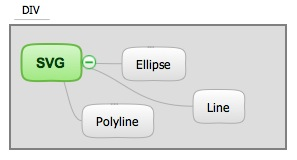
\includegraphics{divsvg.png}
\caption{Esquema del concepto de SVG dentro de un DIV}\label{fig:divsvg}
\end{figure}

Las dos variables a definir son \texttt{mainElem} y \texttt{container}.

\subsection{Implementando}
Todas las funciones de renderizado funcionan de la misma manera. Si se añadiera al código la línea siguiente:
\begin{verbatim}
  <div id="container">
    <v:line from="0,0" to="200,200">
      <v:stroke color="#000000" weight="1" opacity="0.8"/>
    </v:line>
  </div>
\end{verbatim}
se obtendría una línea que iría del punto 0,0 al 200,200 dentro del div contenedor, de color negro (\texttt{\#000000}), de 1 pixel de grosor y una opacidad del 80\%.

Lo que se pretende lograr con el módulo en javascript, es que se pueda ejecutar la línea siguiente:
\begin{verbatim}
  line = new Line(document.getElementById("mainElement"),0,0,200,200,"#000000",1,0.8);
\end{verbatim}
en cualquier momento mediante Javascript, y que automáticamente se cree ese nodo \texttt{<v:line>}. Gracias a que es posible ejecutar código javascript en cualquier evento, es posible crear una línea cuando se pulsa el ratón, e ir modificando sus coordenadas mientras se mueve. No solo eso, sinó que si se recibe alguna información, por ejemplo, mediante Ajax, es posible dibujar dinámicamente elementos a la vez que el servidor los va mandando, sin tener que recargar la página. Es posible usar, por tanto, estas funciones del motor de renderizado tanto para simular el hecho de estar dibujando (motor de dibujo), como para recibir los dibujos que realizan el resto de participantes de una pizarra (módulo de comunicaciones).

Javascript tiene todas las funciones necesarias para modificar el DOM tanto como se desee. Se ha visto que es posible obtener un elemento del código mediante el \texttt{document.getElementById}, y una vez se tiene ese objeto, existen funciones como \texttt{appendChild} para ir modificándolo.

Gracias a jQuery, y a que Javascript es un lenguaje muy relajado sintácticamente, se han podido salvar las distancias entre VML y SVG de forma bastante sencilla. Al final siempre se tiene que implementar cada función dos veces, puesto que la sintaxis de VML y SVG es diferente (hay elementos iguales, pero la sintaxis para crearlos no es la misma), pero estas funciones hacen transparente este proceso. 
